%%%%%%%%%%%%%%%%%%%%%%% file template.tex %%%%%%%%%%%%%%%%%%%%%%%%%
%
% This is a general template file for the LaTeX package SVJour3
% for Springer journals.          Springer Heidelberg 2010/09/16
%
% Copy it to a new file with a new name and use it as the basis
% for your article. Delete % signs as needed.
%
% This template includes a few options for different layouts and
% content for various journals. Please consult a previous issue of
% your journal as needed.
%
%%%%%%%%%%%%%%%%%%%%%%%%%%%%%%%%%%%%%%%%%%%%%%%%%%%%%%%%%%%%%%%%%%%

\RequirePackage{fix-cm}

%\documentclass{svjour3}                     % onecolumn (standard format)
%\documentclass[smallcondensed]{svjour3}     % onecolumn (ditto)
%\documentclass[smallextended]{svjour3}       % onecolumn (second format)
\documentclass[twocolumn]{svjour3}          % twocolumn

\smartqed  % flush right qed marks, e.g. at end of proof

\usepackage{graphicx}
%\usepackage{mathptmx}      % use Times fonts if available on your TeX system
%\usepackage{latexsym}

\journalname{J Comput Aided Mol Des}

\begin{document}

\title{USRT: a de novo Ligand Deduplication and Clustering Algorithm using Ultrafast Shape Recognition with Torsions
%\thanks{Grants or other notes about the article that should go on the front page should be placed here. General acknowledgments should be placed at the end of the article.}
}
%\subtitle{Do you have a subtitle?\\ If so, write it here}

%\titlerunning{Short form of title}        % if too long for running head

\author{Hongjian Li \and Kwong-Sak Leung \and Man-Hon Wong}

%\authorrunning{Short form of author list} % if too long for running head

\institute{Hongjian Li \and Kwong-Sak Leung \and Man-Hon Wong\at
Department of Computer Science and Engineering, Chinese University of Hong Kong, Shatin, New Territories, Hong Kong\\
\email{hjli@cse.cuhk.edu.hk}           %  \\
%\emph{Present address:} of F. Author  %  if needed
%\and
%S. Author \at
%second address
}

\date{Received: date / Accepted: date}
% The correct dates will be entered by the editor

\maketitle

\begin{abstract}

We present the first,
ultrafast
can combine with other USR variants, e.g. USRCAT.

\keywords{de novo ligand design \and deduplication \and clustering \and shape recognition}
% \PACS{PACS code1 \and PACS code2 \and more}
% \subclass{MSC code1 \and MSC code2 \and more} % mathematical subject classification numbers
\end{abstract}

\section{Introduction}

it is necessary to include more than one conformer per compound in the database, since flexible molecules can adopt different shapes, and thus the more of these conformations that are included in the database, the less likely it is to miss molecules with the desired pattern. Could have up to 292 additional conformations \cite{1280}.

The final step for the generation of the test database is to calculate 3D molecular conformations for each of the considered 2D chemical structures. The conformers of a particular molecule are in general geometrically distinct and have low potential energy, as conformers with high internal energy are in principle less likely to occur in Nature. This potential energy is parameterised in what is called a Molecular Mechanics Force Field. In this work, the implementation of MMFF94 [18] provided with MOE [19], a widely used Molecular Modelling software package, is used. MMFF94 has been parameterised for a wide variety of chemical systems of interest to organic and medicinal chemists using computationally derived and experimental data. The high accuracy with which these diverse data could be reproduced by MMFF94 [18] suggests its suitability for small organic molecules. an average of about 200 conformations per compound \cite{1332}.

\cite{1332} no shape method dominates when looking at each target individually, as each method is best in half of the targets. A wide range of factors collectively contribute to the large variability in performance observed across targets. First, errors in the generation of 3D conformers may impact differentially on the top ranked molecules depending on the query molecule and thus on the considered target.

having rotational and translational invariant methods, which are seen as a major advantage. the problematic requirement of aligning molecules for comparison is circumvented, as the proposed distributions are independent of the spatial orientation of database molecules.

Large 3D database, ZINC, istar, 23 million

Given a target protein, hundreds of thousands of ligands are usually docked to find out which one has the highest binding affinity. This method is known as virtual screening. However, the entire drug-like space may contain as many as 10 to the power of 100 molecules, so it is impossible to dock all the available ligands. The de novo ligand design strategy is emerging as a complementary method.

$10^{60}$ drug-like molecules \cite{1104} % Review LEA3D paper

AutoGrow \cite{466}, AutoGrow 3.0 \cite{1354}, iSyn \cite{1381,1387}. They use genetic algorithm. Operators include, mutation, addition, crossover, cutting, selection, etc. Goal is to design ligands that have higher binding affinities. Typical method is to grow an initial scaffold by adding fragments. Any of these types of operators could possibly lead to the generation of duplicate ligands.

In the GA operators, duplicate ligands are occasionally generated. Cumulate generation by generation, and getting sereve. Elitism and fitness proportion in GA not work. Illustrate with two figures, one from iSynMCB, one from crossover (same moieties from different parent ligands, resulting from random mixing, Swap the chemical moieties of known ligands. Link the scaffold and fragment through their respective linker hydrogen atoms).

Selection operator done by iSyn externally calls idock \cite{1153} to evaluate the binding affinity of a population of de novo ligands. It is particularly challenging to tell if two ligands are duplicate when they are in significantly different conformations after being docked against the protein (the selection process) (Figure \ref{fig:MRV}).

\begin{figure*}
\minipage{0.5\textwidth}
\centering
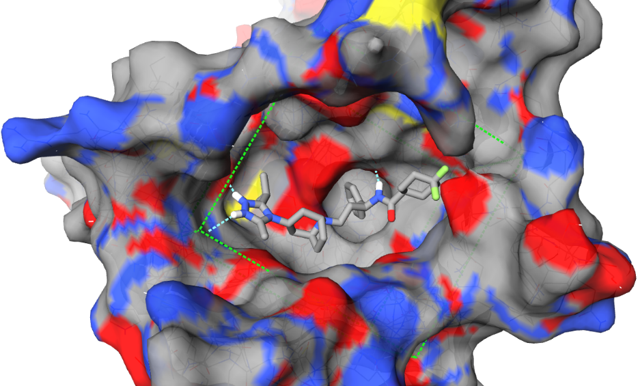
\includegraphics[width=1.36\textwidth,natwidth=638,natheight=386]{../usrt/MRV0.png}
\endminipage
\minipage{0.5\textwidth}
\centering
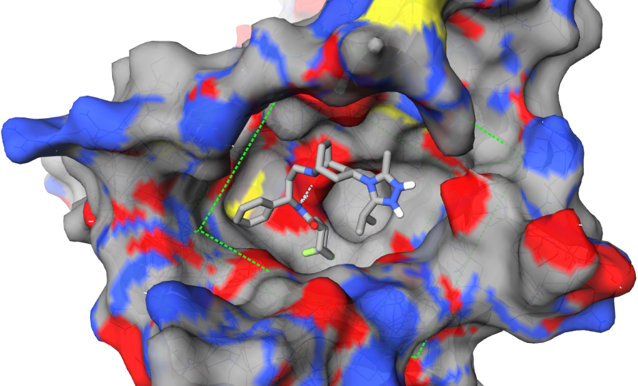
\includegraphics[width=1.36\textwidth,natwidth=638,natheight=386]{../usrt/MRV1.png}
\endminipage
\caption{Two very different docked poses of the marketed HIV drug maraviroc in complex with the human CCR5 chemokine receptor (PDB ID: 4MBS). The protein is rendered in molecular surface representation. The ligand is rendered in stick representation. The binding cavity on the protein surface is depicted by a green cubic box. The putative intermolecular hydrogen bonds are shown as cyan dashed lines. The ligand poses were generated by idock \cite{1153} and the figure was rendered by iview \cite{1366}.}
\label{fig:MRV}
\end{figure*}

Network topology connectivity, SMILES \cite{ or InChi representation, Open Babel \cite{968}
Line notations are linear representations of chemical structures that encode the connection table and usually the stereochemistry of a molecule as a line of text. But they do not encode shape information.

Alignment based methods. Molecular superposition. Precise geometric comparison. Computationally expensive. Similarity score is calculated as the volume overlap.

\cite{1390} used USR for deduplication.

In iSyn \cite{1381,1387}, we used USR \cite{1379,1280}. Much faster, USR finds its applications in retrospective \cite{1332} and prospective \cite{1380} virtual screening. USR is independent of position and orientation, but is dependent on torsions.

\cite{1332} study the ability of USR as a stand-alone method to identify molecules sharing common biological activities through retrospective virtual screening experiments.

There also have been a few extensions of USR developed in recent years to augment the method with descriptors to address the lack of discrimination between enantiomers as well as between compounds having similar shape but different atomic properties. One of the first was a hybrid approach between USR and MACCS key descriptors to add structural properties \cite{1333}. Subsequent extensions tried to tackle the lack of discrimination between chiral compounds \cite{1334,1335}. The latest development has been ElectroShape, a variant of USR that encodes electrostatics and optionally liphophilicity through additional dimensions and centroids \cite{1337,1338}.

USR variants include USR + MACCS \cite{1333}, Chirality CSR \cite{1334}, USR:OptIso \cite{1335}, electrostatics \cite{1337} lipophilicity into ElectroShape \cite{1338}, USRCAT \cite{1331}. The above variants cannot address the duplication issue. One can use ensemble methods like comparing mwt, nha in addition to USR. These are coarse.

\cite{1333} implemented a variant of USR with the first four unbalanced moments of each distribution of atomic distances and incorporated additional chemical information through 2D structural similarity.
\cite{1337} the partial charge defines a fourth coordinate, with atoms being identified by points in four-dimensional space.
\cite{1331} Subset atoms were identified with the help of SMARTS patterns that are used for atom typing in the CREDO database. In the case of an empty subset, for examples if no hydrogen bond donors are found, then the corresponding elements in the moment vector will be set to zero.

\cite{1334,1335} select new centers to distinguish enantiomers.

We present USRT, the first algorithm.

In the following sections, we describe USR and USRT, their execution time.

\section{Methods}

This section introduces USR, USRT.

a new non-superposition based method for molecular shape comparison, called Ultrafast Shape Recognition (USR), has been devised with computational performance at least three orders of magnitude faster than previously existing methods. 

The relative position of the atoms in the molecule is in turn completely determined by the set of all interatomic distances. This is a convenient representation, which directly eliminates any need for alignment or translation, as this set of distances is independent of molecular orientation or position.

the set of all interatomic distances contains more information that is needed to describe accurately the shape of the molecule. This is because the values of these distances are heavily constrained by the forces that hold the atoms together and thus using less information would still provide us with the discriminative power necessary to distinguish between molecules.

The goal is to find different compounds with a shape similar to that of the query, we will direct our attention to the four compounds with the highest score, instead of the four conformers with the highest score. The four conformers with the highest similarity score (top row) to the drug conformer APRD00001-1 from the DrugBank-3D database correspond to four conformations of the same compound, including the query. However, the reason why a database is populated with multiple conformers of each flexible compound is to reduce the possibility of missing compounds with similar shape to the query.

\subsection{USR: Ultrafast Shape Recognition}

USR \cite{1379,1280}

Four reference points, ctd: molecular centroid, cst: closest atom to ctd, fct: farthest atom to ctd, ftf: farthest atom to fct. Compute distances. Moments of these distances have semantics. For instance, the 1st, 2nd, 3rd moments of ctd capture the size, variance, skewness of the ligand, respectively. Applicable to different number of atoms. Dimension reduction: any ligand structure is mapped to a point in a 12 dimensional space. In combination with a suitable clustering algorithm, one could find clusters in a molecular database in order to select the most representative molecule of each cluster. The latter could be applied, for example, as a way to avoid repeating expensive biological tests on similar molecules.  This opens the door to the application of existing clustering algorithms to find groups of similar molecules as a way to analyse the molecular diversity of a database in terms of molecular shape. These roots are intended to provide all moments with linear space dimension, typically Å, in order to avoid differences in high order moments overshadowing the contribution to the similarity score of low order moments.

Dissimilarity transformed into a normalized similarity score. (Eq \ref{eqn:usr}) Inverse monotonic function can do.

\begin{equation}
S_{qi}=\frac{1}{1+\frac{1}{12}\sum_{l=1}^{12}|M_l^q-M_l^i|}
\label{eqn:usr}
\end{equation}

Extensible: reference points, moments

\subsection{USRT: Ultrafast Shape Recognition with Torsions}

PDBQT format, used by AutoDock series \cite{597,596}, Vina \cite{595}, idock \cite{1153}, QVina \cite{1193}. Explain the PDBQT specification (http://autodock.scripps.edu/faqs-help/faq/what-is-the-format-of-a-pdbqt-file).  The structure of a ligand in PDBQT format can be represented by a tree structure of frames, where a frame is the largest connected unit with no rotatable bonds. There are three types of frames: root frame, inner frame, and leaf frame. A root frame has no parent frame and has zero or more child frames. A inner frame has one parent frame and one or more child frames. A leaf frame has one parent frame and no child frames. A ligand must have a root frame, and could have inner or leaf frames.

Ligands can be treated as flexible in AutoDock, and we use the idea of a "torsion tree" to represent the rigid and rotatable pieces. There is always one "root", and zero or more "branches". Branches can be nested. Every branch defines one rotatable bond. The torsion tree is represented in the PDBQT with the following records, and the placement of these records is important, and usually means reordering the ATOM/HETATM records:

Figure \ref{fig:T27} shows two conformations with different torsions. This is a rotatable bond. This branch can rotate along the rotatable bond and flip to the right hand side. A torsion is the rotating angle, so it is in the range of –π to π. 

Reference atom is chosen to be the atom connecting to the parent frame. It is BRANCH X Y, and is often the first of the current frame. For the ROOT frame, it is the first.

\begin{figure*}
\minipage{0.5\textwidth}
\centering
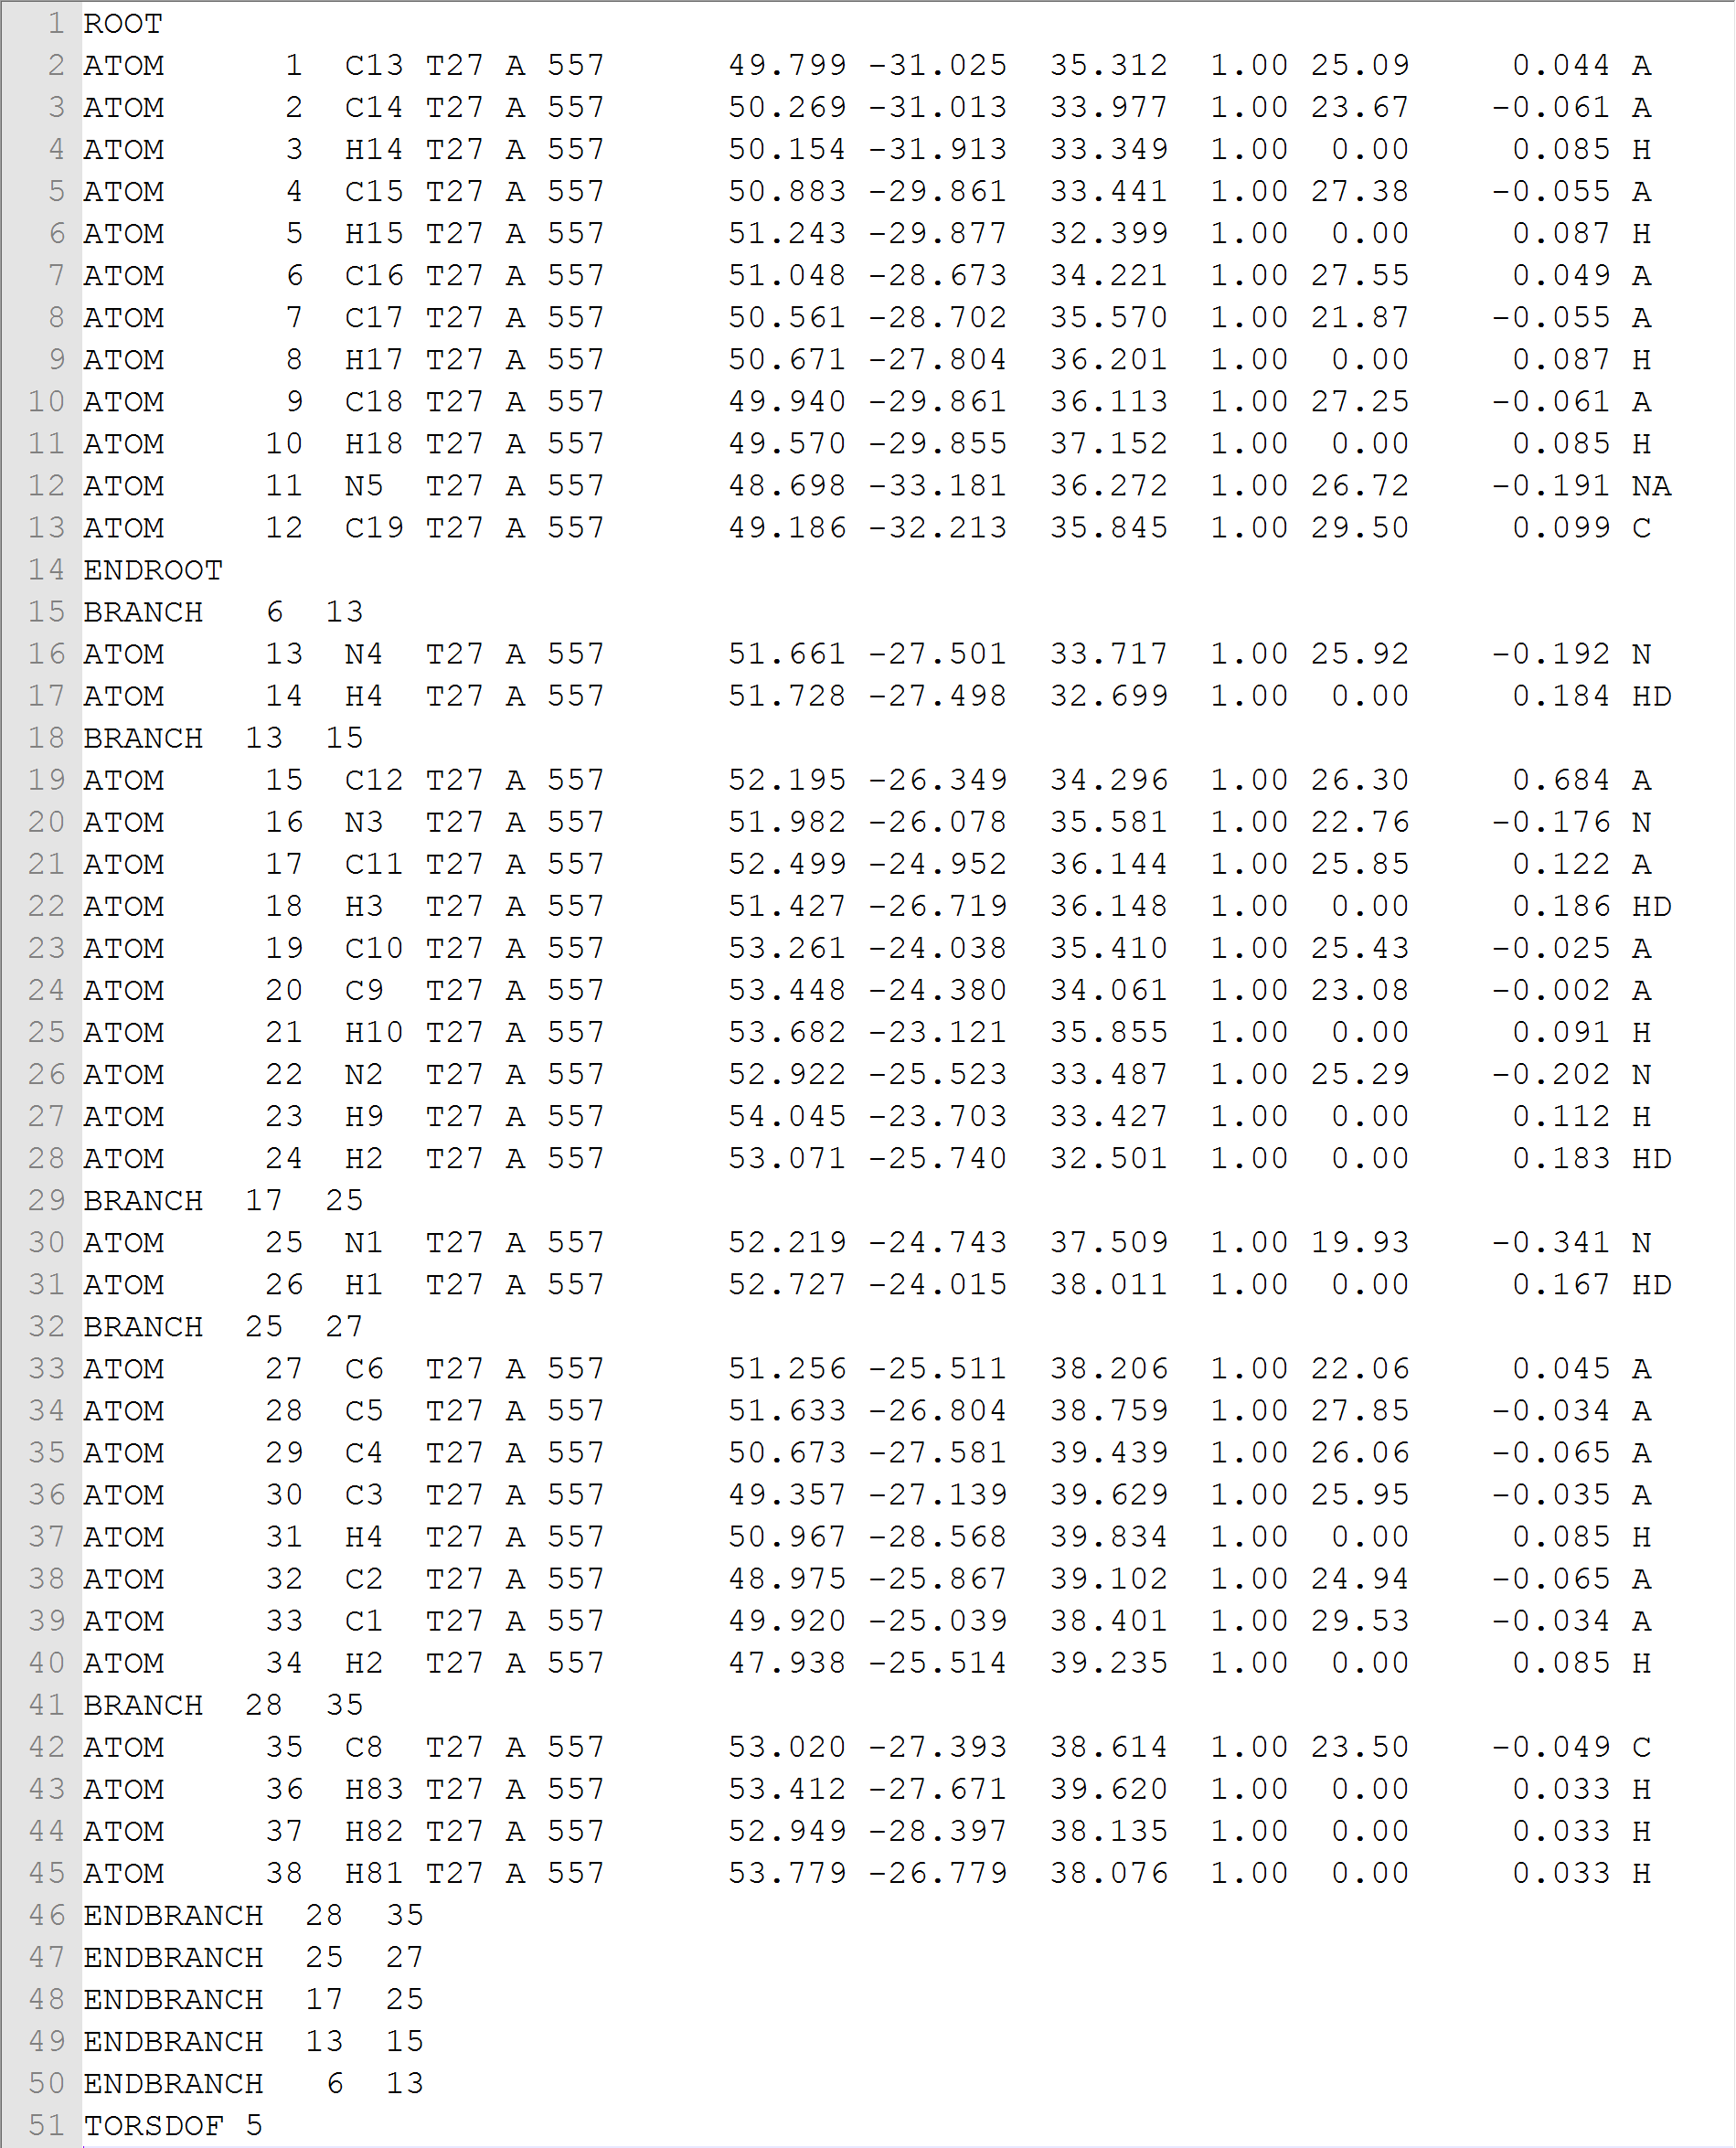
\includegraphics[width=1.36\textwidth,natwidth=1899,natheight=2350]{../usrt/T27CrystalPDBQT.png}
\endminipage
\minipage{0.5\textwidth}
\centering
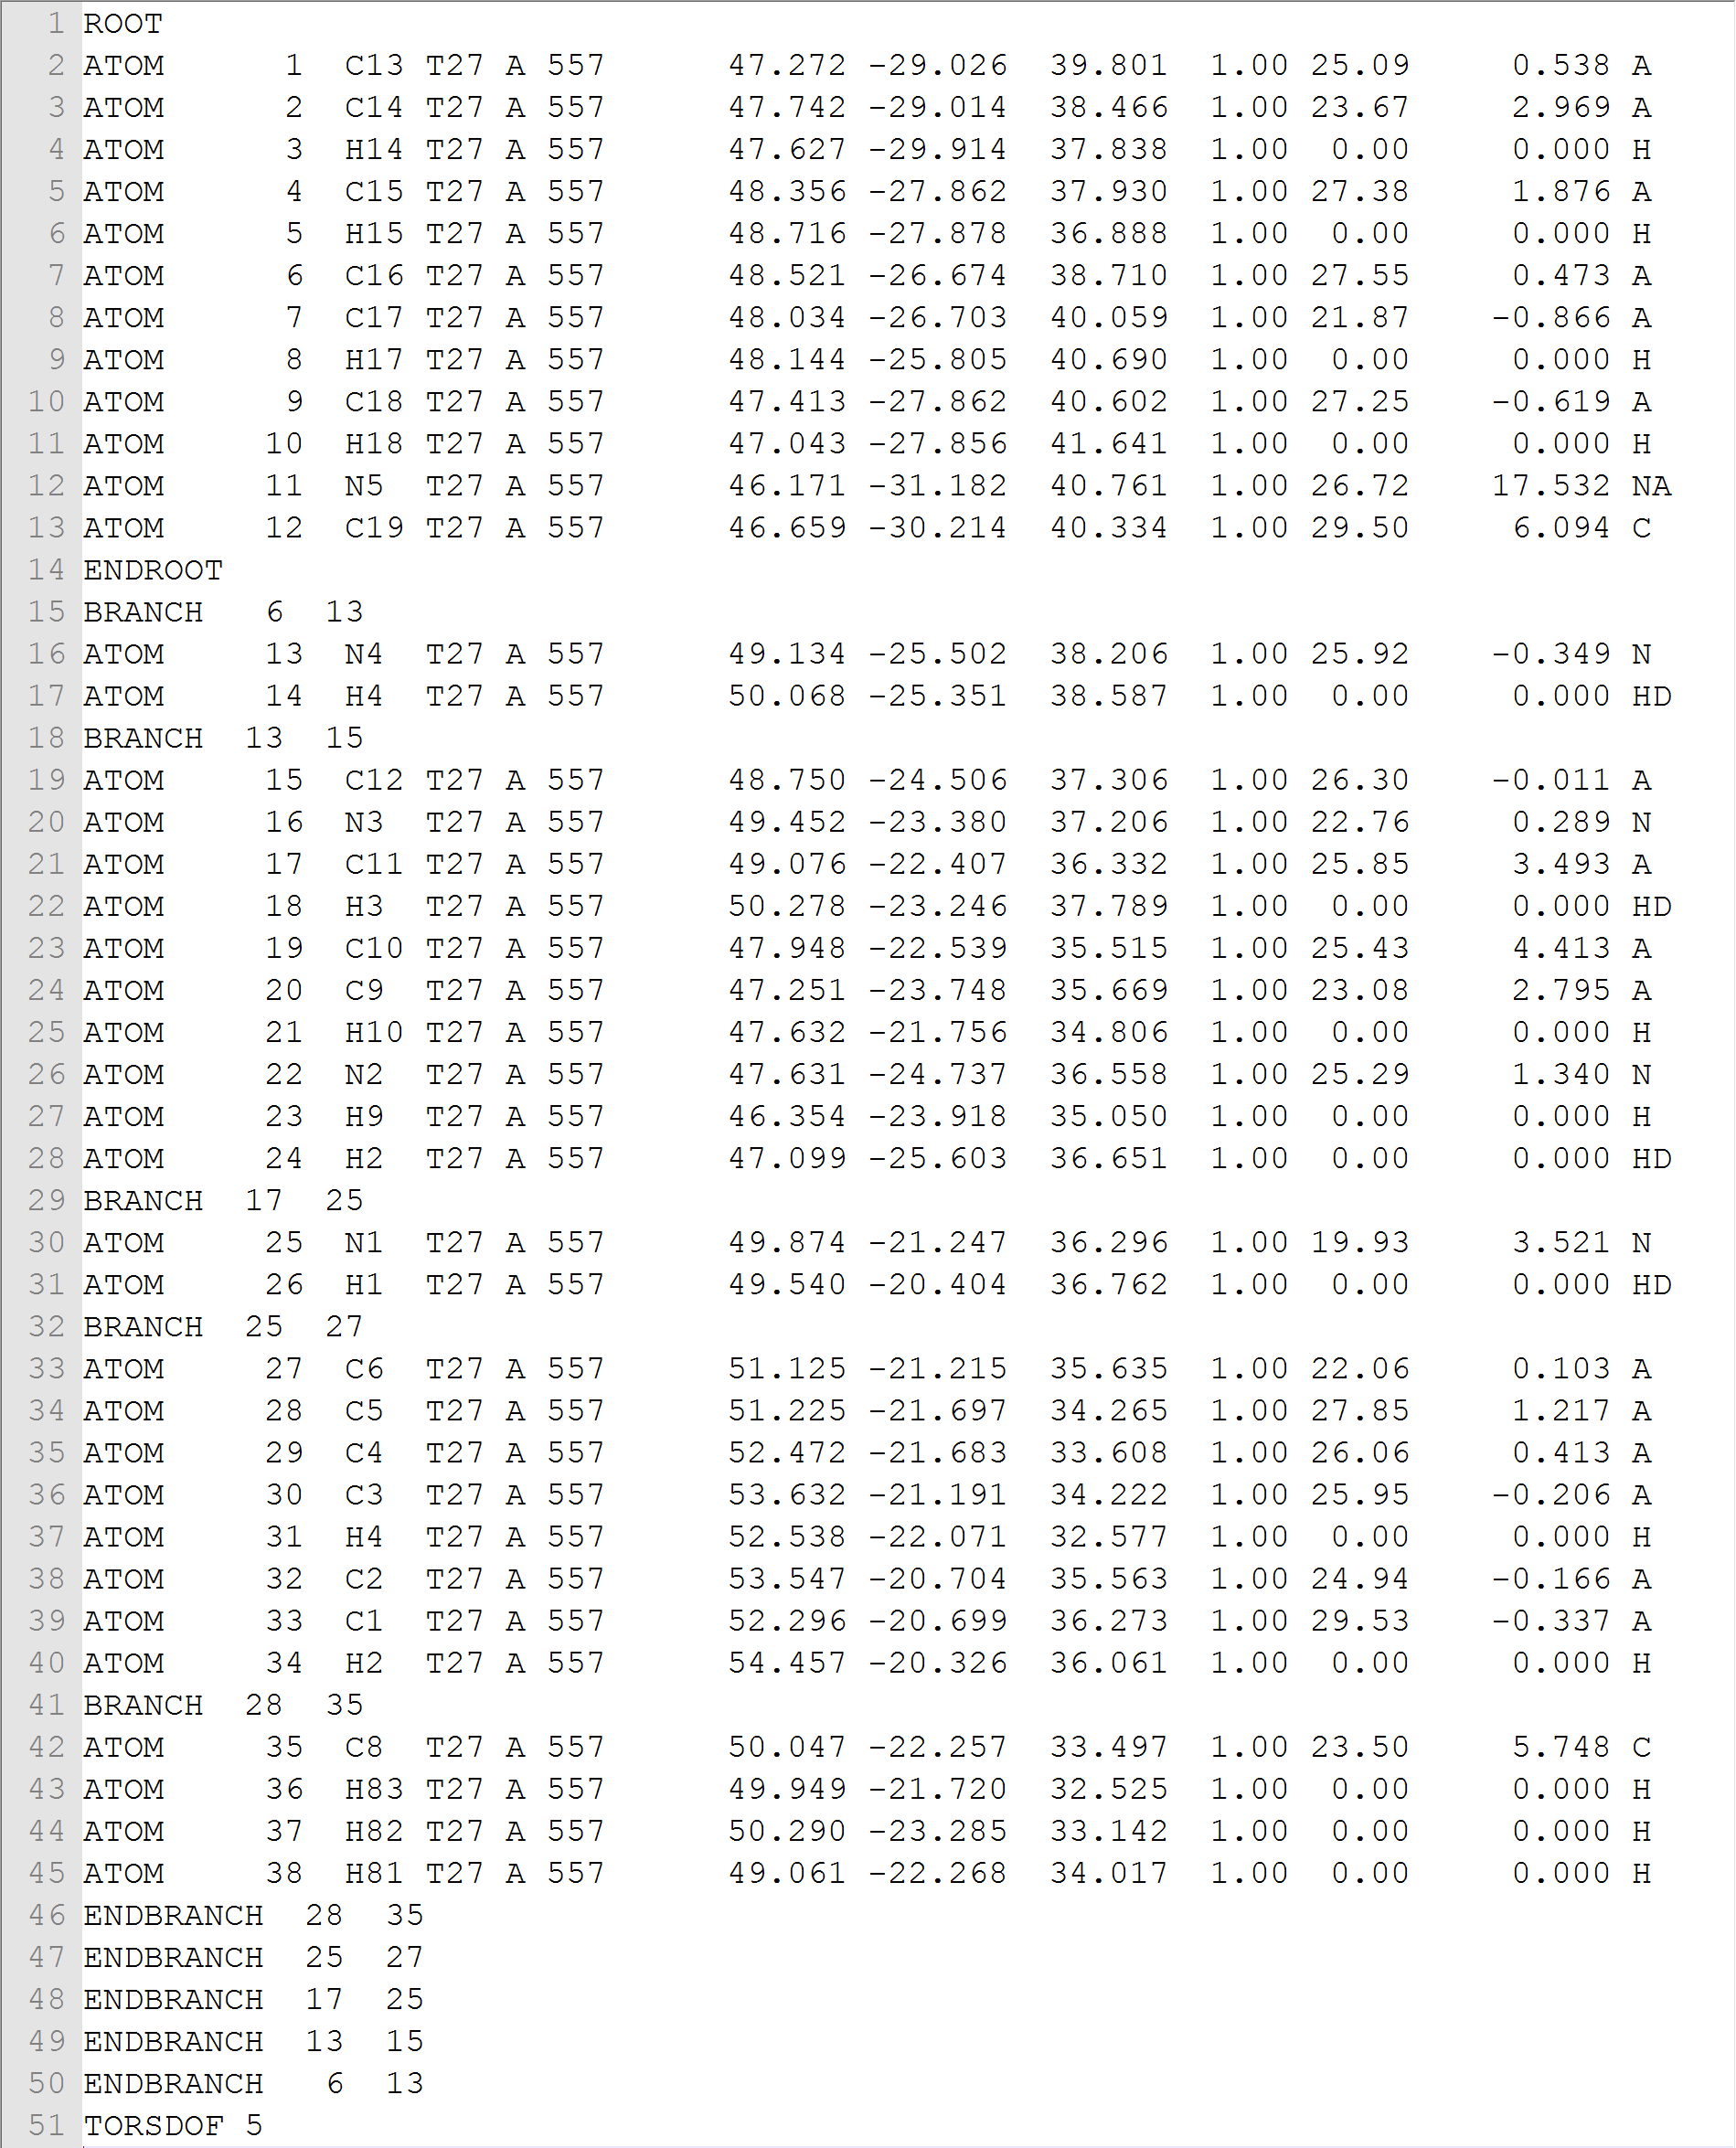
\includegraphics[width=1.36\textwidth,natwidth=1899,natheight=2350]{../usrt/T27DockedPDBQT.png}
\endminipage
\\
\minipage{0.5\textwidth}
\centering
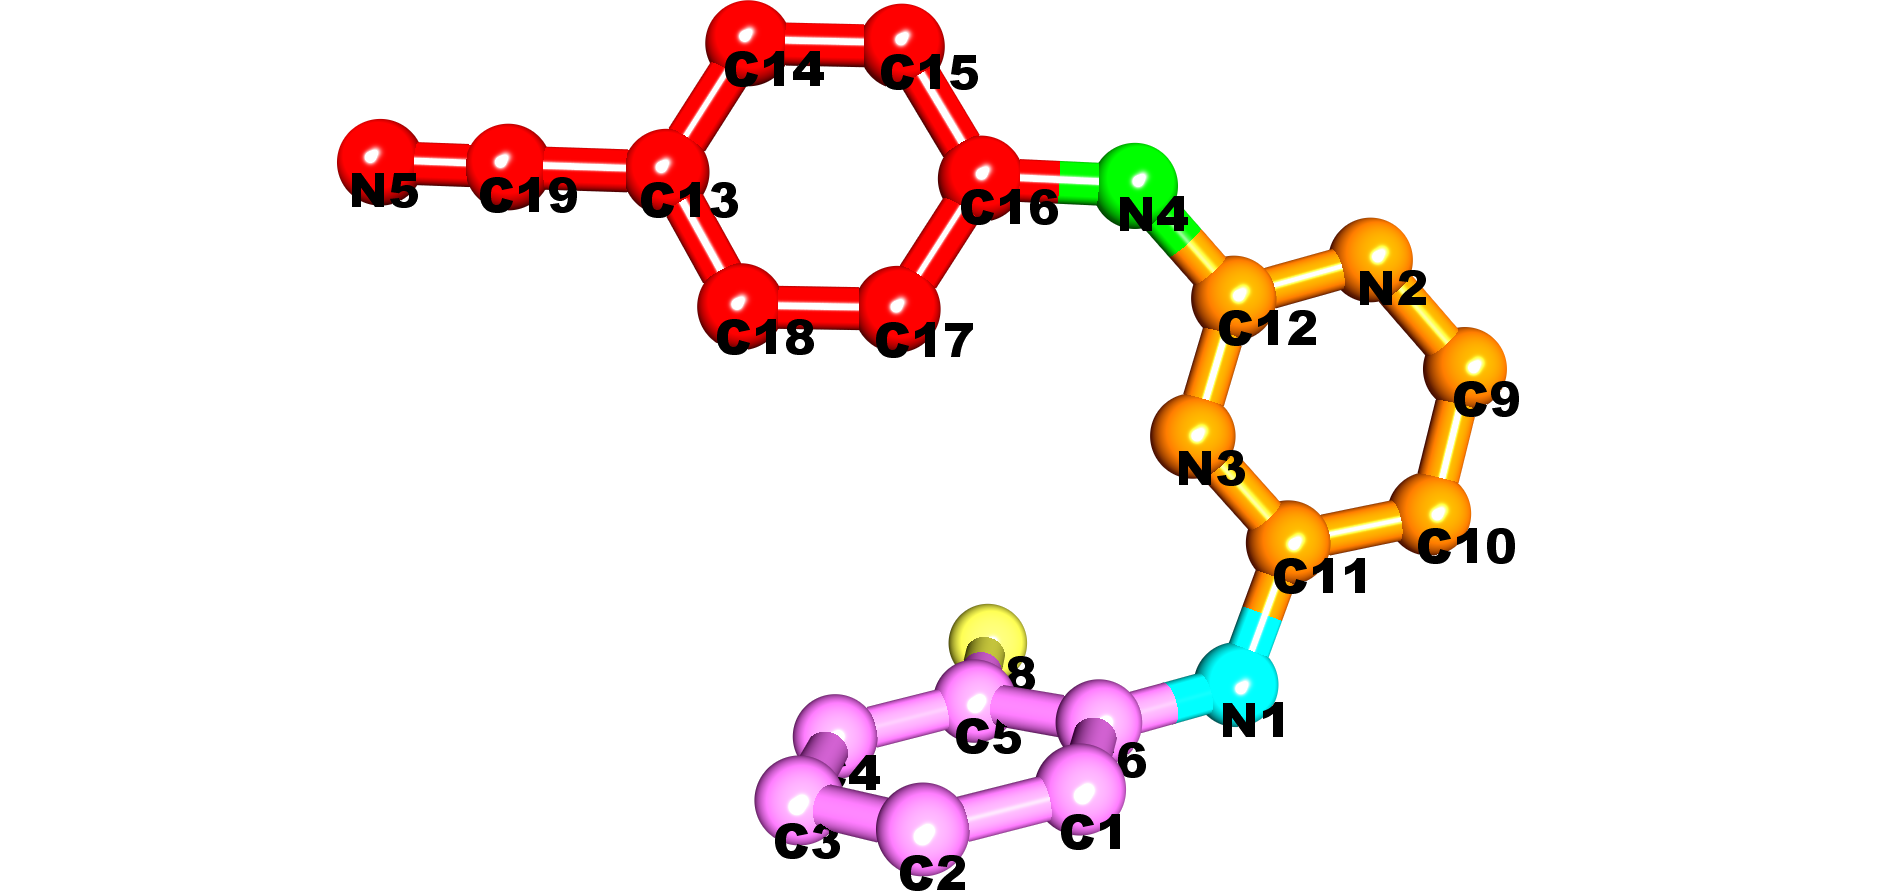
\includegraphics[width=1.36\textwidth,natwidth=1904,natheight=894]{../usrt/T27Crystal.png}
\endminipage
\minipage{0.5\textwidth}
\centering
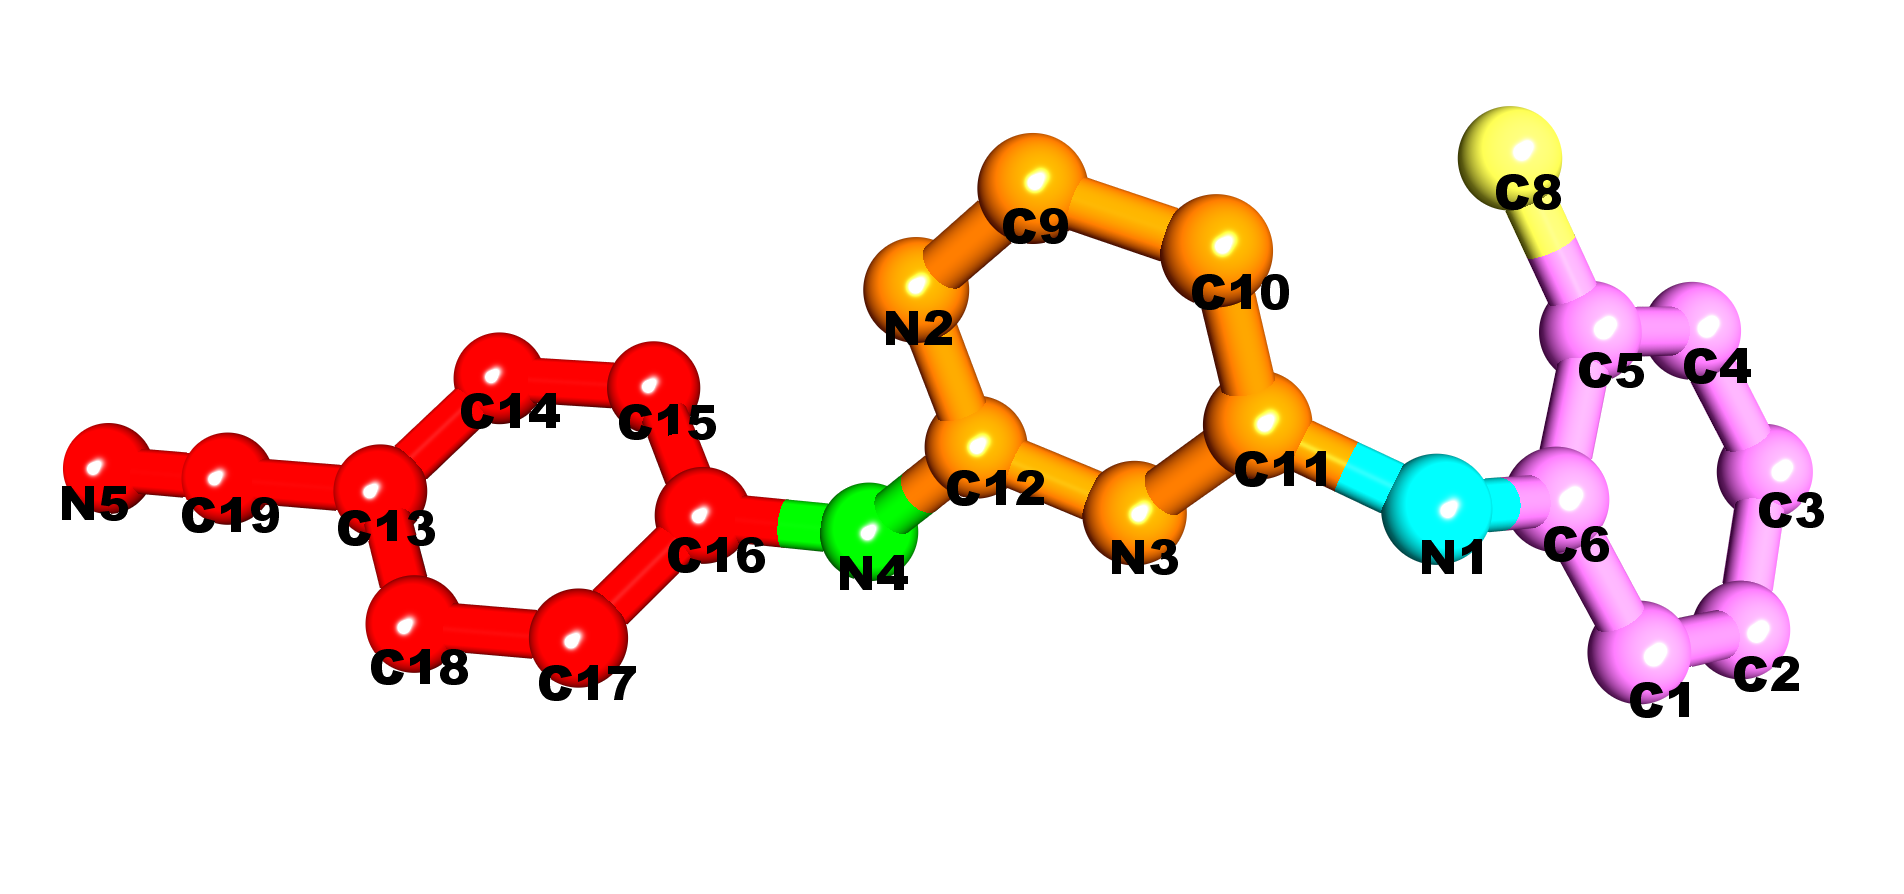
\includegraphics[width=1.36\textwidth,natwidth=1904,natheight=894]{../usrt/T27Docked.png}
\endminipage
\caption{Two very different poses of the same ligand, which has six frames and five rotatable bonds. Top: the contents of the two poses in PDBQT format. Bottom: the two poses in ball-and-stick representation. The atoms and bonds in the same frame are rendered in the same color.}
\label{fig:T27}
\end{figure*}

Once a reference atom is determined, the next is to compute inter-atom distances and their 1st, 2nd, 3rd moments.

Frames with less than 2 heavy atoms are ignored. Could be inactive frames like -CH3, -NH2 or -OH. Cannot compute 2nd and 3rd moments.

\subsection{dbap (N=1,738)}

\subsection{All Clean (N=23,129,083)}

\section{Results and discussion}

\begin{table*}
\caption{USRT output feature vector of the nine poses of the same ligand.}
\label{tab:T27output}
\begin{tabular}{cc}
\hline\noalign{\smallskip}
pose & output vector\\
\noalign{\smallskip}\hline\noalign{\smallskip}
1 & (1.8338,0.9506,-0.8938,1.6928,1.0122,-0.8432,1.7861,1.0556,-0.8661)\\
2 & (1.8338,0.9506,-0.8938,1.6926,1.0121,-0.8433,1.7862,1.0558,-0.8660)\\
3 & (1.8338,0.9506,-0.8938,1.6925,1.0120,-0.8433,1.7868,1.0559,-0.8661)\\
4 & (1.8338,0.9506,-0.8938,1.6930,1.0123,-0.8433,1.7868,1.0561,-0.8661)\\
5 & (1.8338,0.9506,-0.8938,1.6928,1.0122,-0.8432,1.7867,1.0560,-0.8660)\\
6 & (1.8338,0.9506,-0.8938,1.6925,1.0120,-0.8434,1.7870,1.0561,-0.8661)\\
7 & (1.8338,0.9506,-0.8938,1.6930,1.0124,-0.8431,1.7867,1.0560,-0.8660)\\
8 & (1.8338,0.9506,-0.8938,1.6927,1.0121,-0.8434,1.7861,1.0555,-0.8663)\\
9 & (1.8338,0.9506,-0.8938,1.6925,1.0121,-0.8432,1.7868,1.0558,-0.8663)\\
\noalign{\smallskip}\hline
\end{tabular}
\end{table*}

\subsection{Execution time comparison}

USR was claimed to be three orders of magnitude faster than ESshape3D. USR is 1,546 and 2,038 times faster than ESshape3D and Shape Signatures. USR is 14,238 times faster than ROCS, the fastest alignment-based method.

\section{Software availability}

USRT is free and open source under Apache License 2.0. It is available at https://github.com/HongjianLi/usrt and written in C++11. Precompiled executables for 64bit Linux/Windows and examples are provided.

\section{Conclusions and future prospects}

USR has advantages in being independent of position and orientation.

We have developed USRT (Ultrafast Shape Recognition with Torsions), the first algorithm that can distinguish ligands with different torsions. USRT is computationally very fast, independent of torsions. USRT inherits advantages from USR, and is also independent of torsions, which are introduced by flexible ligand docking. It circumvents the need of aligning the molecules before testing for similarity.

Output is a feature vector, which maps to a point in a high dimensional space. All existing clustering algorithms can be utilized.

Emphasize computational efficiency, 3 orders of magnitude faster than ESshape3D, and applicable to large-scale ligand database like istar \cite{1362}, which has collected 23 million ligands from ZINC \cite{532,1178}.

USRT is a general method that can be applied to various drug design applications, including de novo ligand deduplication and clustering. USRT finds its applications in de novo ligand design. Compatible with USRCAT \cite{1331}, +MACCS \cite{1333} and possibly other USR variants \cite{1334}.

No conformers are required. the unbound bioactive conformation could be in principle significantly different from the corresponding bound conformation. No more considerations of using bound or unbound conformations.

The current version of USRT, 1.0.0, has some constraints: known ROOT frame, in-frame atom types, connector atom types. We will address the above limitations in future research. This raises the obvious question of how to compare molecules with different number of torsions.

\section{Author Contributions}

H.L. designed the study, implemented the software, ran the experiments, and wrote the manuscript. All authors discussed results and commented on the manuscript.

\begin{acknowledgements}

This work was supported by the Direct Grant from the Chinese University of Hong Kong and the GRF Grant (Project No. 2150764) from the Research Grants Council of Hong Kong SAR.

\end{acknowledgements}

%\bibliographystyle{spbasic}      % basic style, author-year citations
%\bibliographystyle{spmpsci}      % mathematics and physical sciences
\bibliographystyle{spphys}       % APS-like style for physics
\bibliography{../refworks}   % name your BibTeX data base

\end{document}

%Journal of Computer-Aided Molecular Design 3.172
%Chemical Biology & Drug Design 2.469 
%Molecular Informatics 2.338
%Journal of Molecular Graphics and Modelling 2.325
%IEEE-ACM Transactions on Computational Biology and Bioinformatics 1.616

%Suggested reviewers
%Geoffrey R Hutchison geoffh@pitt.edu, University of Pittsburgh, Department of Chemistry, 219 Parkman Avenue, Pittsburgh, PA 15217, USA
%John J. Irwin, UCSF, jir322@gmail.com
%Jacob Durrant, UCSD, jdurrant@ucsd.edu
%Adrian Schreyer, Department of Biochemistry, University of Cambridge, UK, adrian@schreyer.me
%Matthew R. Reynolds, AIDS Vaccine Research Laboratory, 555 Science Dr., Madison, Wisconsin 53711, mrreynol@wisc.edu
%Masaaki Toyama, Center for chronic viral diseases, Kagoshima University, Kagoshima, Japan, toyama@m2.kufm.kagoshima-u.ac.jp
%Pablo Campomanes, German Research School for Simulation Sciences, p.campomanes@grs-sim.de
%Calvin Yu-Chian Chen, School of Medicine, College of Medicine, China Medical University, Taichung, 540402, Taiwan, ycc929@mit.edu
